\documentclass[11pt]{article}

\usepackage[utf8]{inputenc}
\usepackage{acl2015}
%\usepackage{url}
\usepackage{natbib}
\usepackage{graphicx}
\usepackage{multicol}
\usepackage{hyperref}
\usepackage{threeparttable}
\usepackage{algorithm2e}
\usepackage[toc,page]{appendix}

\title{This Time With Feeling: Sentiment to ML Headlines}

\author{Ben Arnoldy \\
  University of California, Berkeley \\
  {\tt arnoldyb@berkeley.edu} \\\And
  Mark Paluta \\
  University of California, Berkeley \\
  {\tt mpaluta@berkeley.edu} \\}
  
\date{July 2019}

\begin{document}

\maketitle

\begin{abstract}

In this paper we propose a strategy for sentiment-based preprocessing on the task of headline generation. We seek to show that training on sentiment-matched headlines and bodies would result in similar ROUGE scores while simultaneously improving sentiment metrics. Due to resource constraints, we are unable to train to convergence, but our preliminary results support our hypotheses. Training a Universal Transformer on two equivalent data set sizes, one sentiment-matched and one not, we see no noteworthy effect size in ROUGE while seeing improvement of 9\% in our sentiment match between the generated headline and the article lede (first paragraph).
    
\end{abstract}

\section{Introduction}
The art of good headline writing is not as simple as summarizing relevant details; it requires wit, originality, and a tone that matches the piece. Algorithms have made improvements in summarization, but still struggle with these more nuanced elements. Despite this shortcoming, algorithms could still be useful to an editor, suggesting a number of possible headlines to provide inspiration or for the editor to refine and synthesize into a final product. We propose an incremental improvement in automatic headline generation by incorporating tonal bias to match the underlying content.

\section{Background}
Headline generation is primarily approached as a single-document summarization task. The nature of headlines makes them relatively more difficult to produce with machine learning than typical document summaries. First, headlines tend to be shorter than the average sentence, requiring greater concision than typical ML summaries of one or more sentences. Additionally, they are often written in a short-hand style different from the body text, making extractive summarization theoretically less suitable than the more challenging task of abstractive summarization. 

Current methods of summarization involve an encoder-decoder architecture \citep{rush2015neural} with a ROUGE evaluation metric \cite{Ayana2017}. ROUGE is a recall-oriented metric to score a generated summary against a reference summary \cite{lin-2004-rouge}. Specific variants include ROUGE-N, scoring the number of common N-grams, and ROUGE-L, scoring the longest common subsequence. Recent refinements to headline generation include adversarial reward systems to combat repetition \cite{DBLP:journals/corr/abs-1902-07110} and applying state-of-the-art Transformer algorithms \cite{DBLP:journals/corr/abs-1901-07786}.

While most work on headline generation focuses exclusively on summarization, two recent papers in other summarization domains explored efforts to add desired sentiment. One naive approach from Chaudhari et al \cite{DBLP:journals/corr/abs-1802-09426} preprocessed sentences in the body of the corpus to generate sentence-level sentiment scores that characterize the emotional tone of the text. Sentences that did not match the desired sentiment polarity (positive or negative) were dropped before training the summarization model. Another more elaborate approach from Hu et al \cite{DBLP:journals/corr/HuYLSX17} to produce customer review summaries added a discriminator to evaluate the sentiment of generated summaries, looping back to the generator to optimize on this additional criterion. 

\section{Methodology}

\subsection{Objective}
We build a Universal Transformer architecture, initially basing our work off of that of Gavrilov et al \cite{DBLP:journals/corr/abs-1901-07786}, but adding sentiment into the model in the spirit of Chaudhari \cite{DBLP:journals/corr/abs-1802-09426} and Hu \cite{DBLP:journals/corr/HuYLSX17}. To test the effectiveness of adding sentiment, we train an experimental and a control model.

The experimental model trains on the subset of the train dataset where the headline and the first paragraph (i.e. lede) have the same sentiment polarity. This preprocessing results in a reduction in this model's training set from 990,858 articles to 749,745. To ensure that the control model trains on a comparable amount of data, we reduce the control dataset by randomly dropping articles down to 749,745. 

With this approach modeled on Chaudari\cite{DBLP:journals/corr/abs-1802-09426}, our hypothesis is that the experimental model will show improved sentiment matching scores over those from the control model. We evaluate sentiment matching by measuring how many generated headlines have the same sentiment polarity as the first paragraph and, separately, the label headline. We also compare ROUGE scores to see whether this method of improving sentiment matching comes at a cost or benefit to ROUGE score performance.

\subsection{Corpus}
We use the \href{https://catalog.ldc.upenn.edu/LDC2008T19}{New York Times annotated corpus} to match Gavrilov et al. This contains 1.8 million New York Times articles spanning from 1987 to 2006. Like Gavrilov, we filtered out obituaries and retained only articles where $20 \le wordcount \le 2000$ and $3 \le headline length \le 15$. We were left with 1,415,511 articles, which we then split along 70:10:20 proportions into train, dev, and test datasets. We also remove duplicative first paragraphs that occur in many of the articles. 

\subsection{Workflow}

The workflow we defined to preprocess our data can be seen in Figure \ref{figure:preprocess}. Note that as we are running both an experimental group and a control group, the remainder of the workflow can be parallelized across two virtual machines.

\begin{figure*}
  \centering
  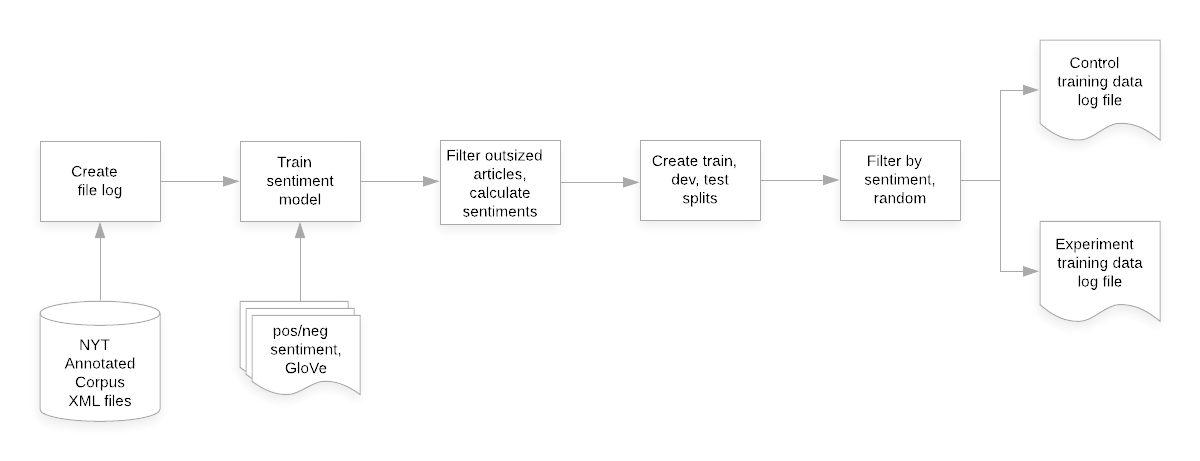
\includegraphics[width=\textwidth]{HeadGen_pre_p.png}
  \caption{Preprocessing workflow}
  \label{figure:preprocess}
\end{figure*}

After preprocessing, the remaining pipeline consists of training, decoding on dev or test data, and scoring decoded output. See Figure \ref{figure:decode} for a full pipeline schematic.

\begin{figure*}
  \centering
  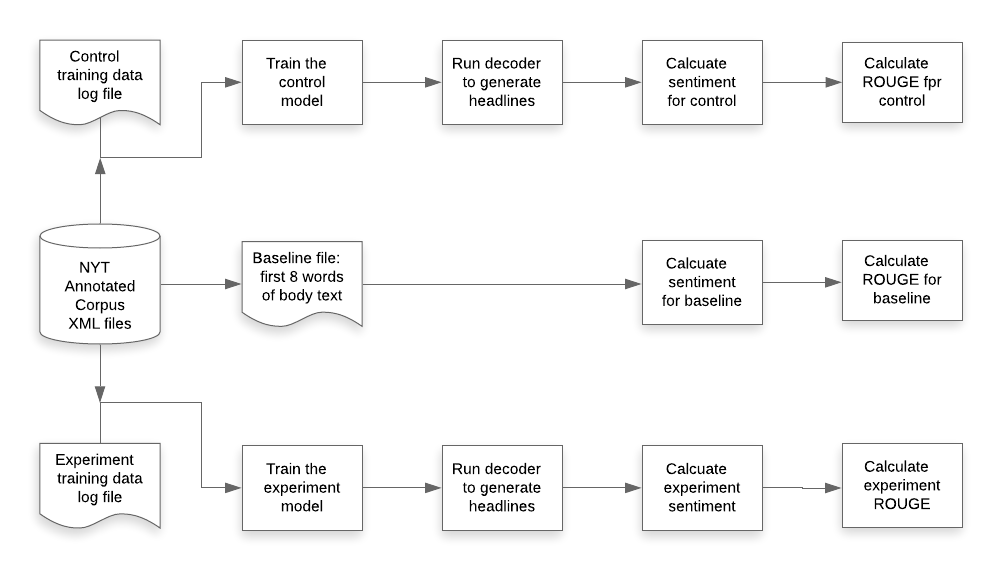
\includegraphics[width=\textwidth]{HeadGen_post_p.png}
  \caption{Train, decode, evaluate workflow}
  \label{figure:decode}
\end{figure*}

\subsection{Implementation of Universal Transformer Architecture}
Specifically, we chose to work with the package \href{https://github.com/tensorflow/tensor2tensor}{\texttt{tensor2tensor}}. This package was developed by the Google Brain team and is designed for furthering research on a variety of natural language processing problems\cite{vaswani-etal-2018-tensor2tensor}. Our explorations indicated that this was the most applicable and flexible package for the task.

We began by replicating the CNN/Daily Mail text summarization problem. We then adapted the architecture to accommodate a new problem of summarization, specifically generating headlines rather than key points, and using the New York Times annotated corpus rather than CNN/Daily Mail. We initially sought to imitate Gavrilov's architecture and results before embarking on our own modifications. This setup included an encoder-decoder architecture, AdamW optimizer, and any specific hyperparameters outlined by Gavrilov, choosing \texttt{tensor2tensor} defaults for anything not specified. Specific adaptations we made in \texttt{tensor2tensor} included:

\begin{itemize}
    \item Preprocess the New York Times corpus to prepare for \texttt{tensor2tensor} ingestion
    \item Define problem \texttt{Gavrilov} inheriting \texttt{Text2TextProblem}
    \item Apply a subword tokenizer to imitate Gavrilov et al's BPE tokenization
    \item Override a variety of default Universal Transformer hyperparameters as defined in Table \ref{table:hparams}
\end{itemize}

Noteworthy parameters are listed in Table \ref{table:hparams}. We also list \texttt{tensor2tensor} base parameters for the Universal Transformer architecture.

\begin{table}[h!]
\centering
\begin{small}
\begin{tabular}{|c |c |c|} 
 \hline
 Hyperparameter & Gavrilov & base \\ [0.5ex] 
 \hline
 Hidden layer size & 1024 & 1024 \\ 
 Filter size & 4096 & 4096 \\
 Heads of attention & 8 & 16 \\
 Layer preprocess sequence & None & normalize \\
 Layer postprocess sequence & dropout & dropout \\
 & $\rightarrow$ add $\rightarrow$ & $\rightarrow$ add \\
 & normalize & \\
 Postprocess dropout & 0.3 & 0.3 \\
 Encoder layers & 4 & 0 \\
 Decoder layers & 4 & 0 \\
 Learning rate warmup steps & 4000 & 8000 \\ [1ex]
 \hline
\end{tabular}
\end{small}
\caption{Hyperparameter Configurations}
\label{table:hparams}
\end{table}

\subsection{Decoder}
Due to the cutting-edge nature of \texttt{tensor2tensor} including limited documentation, the decoder posed a number of initial challenges for us. As mentioned we initially modeled after Gavrilov et al's parameters. However, despite training to 25,000 steps, and numerous experiments adjusting the beam-size, $\alpha$ (length normalization), and the \texttt{decode\_variable} parameter, we almost always got empty output from the decoder. We even adjusted from inputting 10 paragraphs to 3 and retrained entirely to try to downscope the problem and allow for faster convergence, but still encountered the problem. On rare occasions, we were able to get a few words repeated dozens of times. It was unclear to us the reason for our largely blank decoder output, but we suspect it was either a problem in our architecture construction or insufficient training time. Our dev data loss curve also flatlined all the way to 25,000 steps despite decrease in training data loss, which did not bode well.

As a result, we elected to simply try the baseline hyperparameters from \texttt{tensor2tensor}. This approach immediately resulted in notably better performance as we will elaborate on in the results section, so we abandoned trying to imitate Gavrilov et al. Our final chosen parameters for the decoder were $\alpha=0.6$ and $beams=4$ per Vaswani et al \cite{DBLP:journals/corr/VaswaniSPUJGKP17}, and \texttt{decode\_variable} $=100$ based on the default setting.

\subsection{Sentiment analysis}
We use a positive-negative polarity function as most research on sentiment is a simple positive-negative scale and we wish to leverage existing work. Following a model produced and annotated by Speer\cite{RacistAI}, we take Liu's opinion lexicon\cite{Hu:2004:MSC:1014052.1014073} -- a list of around 6,800 words that are labeled either positive or negative -- and embed the lexicon's words in pre-trained GloVe embeddings. These embeddings and their [0,1] labels are used to train a logistic regression model that returns the log probability of a new word being positive and the log probability of it being negative. The negative probability is subtracted from the positive to arrive at a score; positive scores indicate positive associations and vice versa. To score an entire headline, we take a bag of words approach and sum the individual scores of all the words in the headline and take an average. We construct a filter to remove articles where the polarity of the headline and its short summary differ.

\subsection{Evaluation} To test the quality of generated headlines, we ran the first three paragraphs of the body text of the test set articles through the decoder to generate headlines to evaluate the quality of the sentiment-filtered model and the control model. We chose the first three paragraphs after first trying to take the first 10 paragraphs and finding that training and decoding would take too long. We arrived at three by relying on domain knowledge. One of the authors has worked for two decades as a journalist; in traditional news-writing, the first three paragraphs usually contain all the key facts and a "nut graf" that lays out why the story is important. 

Our evaluation included both the standard ROUGE metrics used for summarization tasks as well as two measures of sentiment we designed. The decoding proved computationally intensive and we had to evaluate on a limited test set of 500 examples instead of the full ~280,000 as we originally intended. For more information on resource consumption, see Appendix A.

To compare the two models' performance on sentiment, we first calculate the percentage of generated headlines that match the polarity of the first paragraph of the body text. We call this \%-match-lede, and we treat it as an expression of each model's ability to generate headlines that fit the sentiment of their articles. We also calculate the percentage of generated headlines that match the polarity of the label headline. We call this \%-match-hede, and we treat it as an expression of each model's ability to match the sentiment of the gold standard headline. 

We expect that the preprocess filtering by sentiment will result in a trained model that produces higher \%-match-lede and \%-match-hede scores. 

We developed and ultimately discarded other possible sentiment metrics including f1-scores and differences in raw sentiment scores between generated and label headlines. We discarded the former as less understandable than our metrics and discarded the latter as misleading in their precision given the simplistic nature of the sentiment scoring model.

We also compare to a baseline algorithm of the first eight words of the article. This is based on an average headline word count of 7.52 in our training data.

\section{Results}

Three example input-output pairings are shown in Table \ref{table:example}.

\begin{table}[h!]
\centering
\begin{tiny}
\begin{tabular}{|p{7cm}|} 

 \hline
 \textbf{Input:}The Bush administration asked a federal claims court today to seal documents relating to hundreds of claims that a mercury-based preservative in vaccines, thimerosal, has caused autism and other neurological disorders in children. Lawyers for the Justice Department asked for the protective order on behalf of Tommy G. Thompson, the secretary of health and human services, whose department administers a government fund to compensate people injured by vaccines. A department spokesman said that the law creating the fund gives the secretary control over what information is released and that the government was merely trying to preserve that right.
 \\ [0.5ex] 
 \hline
 \textbf{Output - Baseline:}The Bush administration asked a federal claims court
 
 \textbf{Output - Control:}U.S. Appeals Court Upholds Tobacco Ban

 \textbf{Output - Experiment:}U.S. Says It's Not to Pay for AIDS \\ 
 \hline
 \hline
 \textbf{Input:} To the Editor: If it were decided that the human embryos whose destinies are being weighed (letters, July 18) are indeed living persons, I would hope that a way could be found to give meaning to those lives. I would find greater meaning in having my life used in research that might help to save other lives than in being confined to a slow, purposeless death in cold storage. NANCY S. DORFMAN  Belmont, Mass., July 18, 2001 \\ [0.5ex] 
 \hline
 \textbf{Output - Baseline:}To the Editor: If it were decided that
 
 \textbf{Output - Control:}What's Time to Do It

 \textbf{Output - Experiment:}The Way We Live Now \\ 
 \hline
 \hline
 \textbf{Input:} The Rangers' season could hinge on the magnetic resonance imaging test that Pavel Bure is scheduled to have today. Bure, who is considered by many the best pure goal scorer in the National Hockey League, was injured when his left knee struck the knee of the Sabres' Curtis Brown nine minutes into the second period of the Rangers' 4-1 loss to the Buffalo Sabres last night at Madison Square Garden. For the second time in less than 24 hours, the Rangers -- who lost, 3-2, in overtime in Philadelphia on Thursday night -- failed to move above .500 for the first time since opening night. \\ [0.5ex] 
 \hline
 \textbf{Output - Baseline:}The Rangers' season could hinge on the magnetic
 
 \textbf{Output - Control:}Rangers' Defense Is Back

 \textbf{Output - Experiment:}Devils' Defense \\ 
 \hline
\end{tabular}
\end{tiny}
\caption{Example Output}
\label{table:example}
\end{table}

We ran our algorithm for 25,000 steps as defined within \texttt{tensor2tensor}. For reference, the package recommended running machine translation tasks for approximately 300,000 steps to converge and obtain state-of-the-art BLEU scores. We were unable to run fully to convergence due to resource constraints. For further information about computation times, see Appendix A. Our loss curves are shown in Figure \ref{figure:loss}. Note that due to resource constraints we were also unable to continue evaluation on our dev data past 4000 steps due to the high computational cost of evaluation. We do note that the loss on our dev data was decreasing for the interval on which we were able to evaluate, which was an early indication that the algorithm was generalizing beyond the training data and not simply overfitting.

\begin{figure}
  \centering
  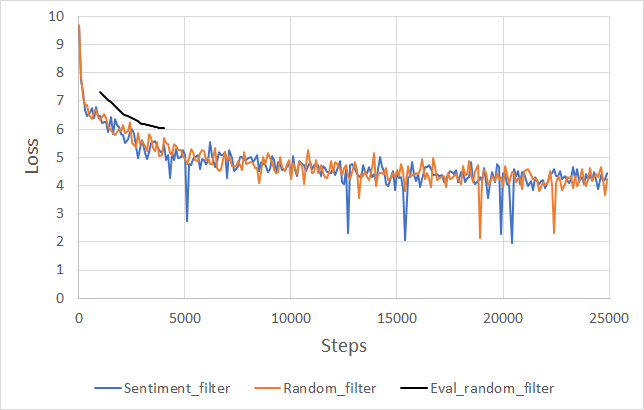
\includegraphics[width=7.8cm]{loss.png}
  \caption{Loss curves}
  \label{figure:loss}
\end{figure}

Given the decoder challenges, we abandoned the Universal Transformer hyperparameters outlined in Gavrilov and instead worked with preset Universal Transformer hyperparameters provided in Tensor2Tensor. This resulted in decoder output good enough to obtain meaningful ROUGE metrics and sentiment metrics. 

Results from our Universal Transformer and Gavrilov's reported scores can be seen in Table \ref{table:results}. 

\begin{table*}[h!]
\begin{threeparttable}
\centering
\begin{small}
\begin{tabular}{|p{7cm}|p{.8cm}|p{.8cm}|p{.8cm}|p{.8cm}|p{.8cm}|p{.8cm}|p{1cm}|p{1cm}|}
 \hline
 Model & R-1-f & R-1-r & R-2-f & R-2-r & R-L-f & R-L-r & \%-match-lede & \%-match-hede \\
 \hline
 Gavrilov Universal Transformer - unsmoothed & \textbf{26.86} & 25.33 & \textbf{13.48} & \textbf{13.01} & \textbf{24.84} & 24.38 & - & - \\ [0.5ex] 
 Gavrilov baseline (first sentence) & 11.64 & \textbf{34.67} & 2.28 & 7.43 & 7.19 & \textbf{31.39} & - & - \\ 
 Our baseline (first 8 words) & 7.74 & 8.39 & 1.67 & 1.69 & 7.12 & 8.16 & 76 & 72.2\\
 Our Universal Transformer - Sentiment-filtered & 10.39$^{*}$ & 9.62$^{*}$ & 6.33$^{*}$ & 5.86$^{*}$ & 9.30$^{*}$ & 9.54$^{*}$ & \textbf{91}$^{*}$ & \textbf{74}$^{*}$ \\
 Our Universal Transformer - Randomly filtered & 10.44$^{*}$ & 9.69$^{*}$ & 6.21$^{*}$ & 5.94$^{*}$ & 9.87$^{*}$ & 9.64$^{*}$ & 80$^{*}$ & 71$^{*}$ \\ [1ex]
 \hline
\end{tabular}
\end{small}
\begin{tablenotes}\footnotesize
\item[*] Note: not trained to convergence and scored on limited test set
\end{tablenotes}
\caption{Results}
\end{threeparttable}
\label{table:results}
\end{table*}

\section{Discussion}

As expected, we saw similar ROUGE metrics across the board and slightly improved sentiment metrics for the experimental model. This signals that the development of more complex integrations of sentiment into headline summarization models would be a worthwhile avenue for future research.

We also observe that Gavrilov's first sentence baseline exhibits better ROUGE recall than our first eight words. We attribute this to the fact that the average journalistic first sentence is substantially longer than eight words and thus their baseline is practically guaranteed to recall more of the headline's words than our baseline.

Although our methodology did show an improvement in our sentiment metrics, we also note that this experiment required throwing out training data. In any real-world headline generation application, it is unlikely that one would want to throw out training data if the primary task is summarization. To measure the effect on ROUGE of throwing out this data, we initially wanted to also run a third model with no downsampling after the initial filtering. This would additionally demonstrate the loss in ROUGE due to decreased training set size, but we did not have enough time to pursue this third model.

The sample generated headlines in Table \ref{table:example} show both the limitations of undertraining headline summarization models and points to some promising improvements with sentiment matching. In all three of these examples, both the control and the experiment models generate factually incorrect headlines. However, we observe that the experiment model's headlines in the first two examples are more reflective of the input text sentiment. In the first example, the input text dwells on childhood diseases, efforts to seal documents, and a federal agency wielding its control over information. 

The control headline misses the tone with the choice of "upholds" as the key verb, while the experiment headline zeros in on the negative phrasing "not to pay." In the second example, an intense input text that grapples with the meaning of life gets the more emotionally resonate headline from the experiment model -- "The Way We Live Now" -- than the control -- "What's Time to Do It." 

The third example highlights one of the pitfalls of this simplistic use of sentiment scoring. The input describes the Rangers, a pro-hockey team, losing a game and facing the loss of a key player due to injury. The experimental model's headline substitutes an entirely different team -- the Devils -- potentially in an effort to match the negative polarity of the input with a team name that has negative sentiment (for reasons beyond sports). We saw other examples of the wrong teams being placed in the experiment model's headlines, including dropping the Yankees in favor of the Mets. Apparently, after being trained on GloVe embeddings, the sentiment model ranked the Yankees extremely negatively (-8.04) compared to the Mets (-4.49) and the model was possibly trying to temper the negativity of the headline.  

Further work could also consider a more sophisticated sentiment analysis than a bag of words approach. We chose to use a simple approach for proof of concept, but one idea for a next iteration could be the \href{https://nlp.stanford.edu/sentiment/index.html}{Stanford Sentiment Treebank}. Rather than throw out training data, another approach could be to utilize a compound loss function incorporating sentiment mismatch in addition to perplexity. A final consideration could be more filtering of undesirable data on the front-end. We noticed for example that there were some "articles" that were simply stock market reportings, which are not reflective of the average newspaper headline.

\section{Conclusion}
In this study, we observe preliminary results that indicate that sentiment-matched newspaper headline and bodies may yield better sentiment properties during headline generation, while sacrificing little in the way of ROUGE when compared to a similar data set size without sentiment match. However, our conclusions are drawn before convergence and on a limited test set, so we recommend follow-on research confirm these trends continue. We also recognize that throwing away training data may yield lower ROUGE scores, so we additionally recommend research on a data set without any downsampling to understand the effect of throwing out this data.

\section{Materials}
Our materials for this project can be found at the following link:
\url{https://github.com/mpaluta/headline_generation}.

% "citing Rush here" \citep{rush2015neural}
% "citing Ayana here" \cite{Ayana2017}
% "citing Peng Xu here" \cite{DBLP:journals/corr/abs-1902-07110}
% "citing Gavrilov here" \cite{DBLP:journals/corr/abs-1901-07786}
% "citing Chaudari here" \cite{DBLP:journals/corr/abs-1802-09426}
% "citing Zhiting Hu here" \cite{DBLP:journals/corr/HuYLSX17}
% "citing Lin here" \cite{lin-2004-rouge}
% "citing Attention is all you Need here" \cite{DBLP:journals/corr/VaswaniSPUJGKP17}

\bibliographystyle{plain}
\bibliography{references}

\begin{appendices}

\section{Resource Considerations}

As we ran our algorithm on several different resource configurations, we decided to take the opportunity to record approximate computation times on various configurations to inform future resource requirements for future work, as some results were nonintuitive. Our approximate benchmarks can be seen in Table 4.

\begin{table}[h!]
\begin{threeparttable}
\centering
\begin{small}
\begin{tabular}{|p{2.6cm}|p{2.2cm}|p{2cm}|} 
 \hline
 Task & Configuration & Approx. Computation Time \\ [0.5ex] 
 \hline\hline
 Vocab Generation & CPU-heavy$^{1}$ & 5 hr 40 min \\ 
  & Balanced$^{2}$ & 40 min \\
  & GPU-heavy$^{3}$ & ? \\
 \hline
 One training step & CPU-heavy & 3.9 sec \\
  & Balanced & 9.7 sec \\ 
  & GPU-heavy & 12.7 sec \\[1ex]
 \hline
 Decode one file & CPU-heavy & 1 min \\
  & Balanced & ? \\ 
  & GPU-heavy & 1 min 30 sec  \\[1ex]
 \hline
\end{tabular}
\end{small}
\begin{tablenotes}\footnotesize
\item[1] 32 vCPUs on Google Cloud
\item[2] Nvidia 1060 GPU and Ryzen 7 2700 (8 cores, 16 threads)
\item[3] 8 vCPUs and Nvidia Tesla K80 on Google Cloud
\end{tablenotes}
\caption{Computational Benchmarks}
\end{threeparttable}
\label{table:hardware}
\end{table}

Of particular note, we observed that vocabulary generation was a GPU-intensive task and benefited greatly from the addition of a GPU. On the other hand, training was CPU-bottlenecked and even a competitive GPU with eight vCPUs was outperformed by just 16 vCPUs with no GPU. This result in particular was surprising and led us to perform most of our intensive training on CPU-heavy configurations. Decoding time appeared to be slow on both CPU and GPU configurations.

\end{appendices}

\end{document}



